%2.1 -- INITIAL REVISIONS MADE
\section{Introduction}
\paragraph{}
Within this chapter, we share an overview of the problem pertaining to the library resource's mobile capabilities, academic and otherwise. We will describe the pros and cons, as well as the possible solutions. Next, we delineate best practices related to mobile application development that have been refined and certified by experts within this field. To conclude, we introduce the requirements to develop a mobile application from the ground up.


%2.2 -- INITIAL REVISIONS MADE
\section{Significance of the Topic}
\paragraph{}
 Our world is becoming more and more reliant on devices such as our mobile phones. These mobile devices unlock a connection between the user and a vast and seemingly endless supply of helpful and sometimes not so helpful resources. With this in mind, this connective architecture, according to Yip et al., "serves as a virtual platform for learners to engage with their learning activities in a more spontaneous, personal, informal, contextual, portable, ubiquitous and pervasive way" (2021, p. 389). Mobile applications are greatly utilized in the academic world on all levels. From elementary school to college graduate students, such applications aid each one to some extent, broadening their learning capabilities and resources.
 
 \paragraph{}
 Mobile apps can often emulate desktop-based websites, but are streamlined in comparison. The use of this is to take a website that is accessible through a desktop or laptop and enable the same or more stark access to the same website. While developing a mobile website that could house the resources of a library may be a more simple task, it leaves for less capabilities and utilities for the mobile user. Developing a native application that can support any mobile platform is a more daunting task, however, the results are of a much higher quality in the end. The user experience in this case is far superior to that of a website (Margam \& Saleeq, 2017, p. 110).
 
\paragraph{}
 Shih-Chuan Chen states, based on the results from a survey of undergraduate students, "Many libraries provide mobile app services because of the rapid increase in smartphone users" (2019, p. 731). He also goes on to note how many elementary tasks are accomplished more efficiently on a mobile device than on a computer, however, the inverse is true for tasks that require the use of searching and web browsing. Laptops and desktops alike were proven to supersede mobile devices in this case, however, mobile devices are still useful for these tasks. This survey shows that, having academic options such as mobile resources that are engaging and user friendly could negate the necessity of in-person attendance to a library or other academic facility. Certain resources such as occupancy tracking, tech suite booking, library hours, and others would not only help students to use their time more efficiently, and potentially reduce the number of people in the library and thereby help follow any local social distancing guidelines in a safer manner.
 
 \paragraph{}
 After all, we live in a time where convenience is of utmost importance. No one of us desires to wait for access to something we need to use. It is a natural human behavior. Technology has amplified that mentality as it provides its users relatively instant access to just about anything at anytime (Shahriza et al., 2006).

\paragraph{}
When developing a mobile application, many factors have to be considered well in advance before code starts to be structured and written. For example, a native application is typically developed to be supported on a specific device platform such as IOS devices. Thus, when developing a mobile app, additional steps need to be taken to include the possibility that the app can be supported by all or most other mobile devices as well. After development, the application will need to be verified and reviewed by the various app stores, i.e. Android's Google Play Store and Apple's App Store, to be displayed and downloadable for any user on each respective platform. Since the application is intended to be public and accessible by many, it has to be run on a network server (Huy \& vanThang, 2012, p. 25-26). These App stores have a significant amount of user traffic, and billions of application downloads and dollars in revenue have transpired on just the Apple App and Google Play stores. These conditions make for a seriously competitive industry (Wang et al., 2017, p. 163).

\paragraph{}
Acknowledging the features a mobile application should embody can be relatively easy, but determining the delivery format and final product in which the user consumes such an app is far more difficult. In a study conducted by Ngu Phuc Huy from Norwegian University of Science and Technology and Do vanThanh from Telenor \& Norwegian University of Science and Technology, four different types of mobile app paradigms were analyzed: Mobile native applications, Mobile widgets, Mobile Web applications, and HTML5 mobile applications. From their research, Huy and vanThanh devised what they called "Evaluation Criteria" (\url{https://doi.org/10.1145/2428955.2428968}) which outlines a rigorous and detailed template for mobile app development (2012, p. 26-27). This evaluation criteria spells out the necessary steps, some perhaps unnecessary in some cases, that aid a developer in structuring and designing a mobile application. Each criterion is carefully considered in the development process to deliver a product to the selected demographic in the best and most effective way possible.



%2.3 -- INITIAL REVISIONS MADE
\section{Known and Unknowns}

    \paragraph{}
    Any experienced programmer can effortlessly throw together a quick application, but developing a user-facing application that people will want to use is entirely another beast. A development team requires more resources, such as designers for the look-and-feel of a mobile application. This also applies to the development of a mobile library application. According to Saragossi et al., "the adoption of mobile apps as an emerging format within the Libraries’ collections necessitates a varied outreach strategy that endeavors to make apps accessible and approachable" (2018, p. 202). So, how does one design and implement an accessible and approachable mobile application? Through research. This research includes, surveys and credible sources to provide evidence and a concrete background that will lead the reader to the point in which the team's work will embark.
    
    Shih-chuan Chen, a professor of Library and Information Sciences, researched the potential benefits for students when using mobile applications to search library catalogs. The study "demonstrates that the participants spent more time completing tasks while using the laptop than that they did while using the mobile app" (Chen, 2019, p. 727). This research clearly shows that users can be more efficient on a mobile device, specifically in the case of utilizing academic library resources.
    
    However, not all features of applications are best used on mobile devices. For example, the same study proved that: \begin{quote} ten participants [out of 16 undergraduate students] reported that it was easier to search the library catalog using the laptop. They explained that they were familiar with the interface of web OPACs [library catalog], and more information was displayed. Moreover, the web OPAC offered more functions. (Chen, 2019, p. 728)\end{quote}
    
    
 %2.4 -- INITIAL REVISIONS MADE
\section{Current Models in This Field of Study}
    \paragraph{}
    A 2018 study by Mansouri and  Soleymani, investigated the necessary features for a library mobile application. The research was performed at the University of Isfahan, known for science, humanities, and engineering.
    \begin{figure}[H]
        \centering
        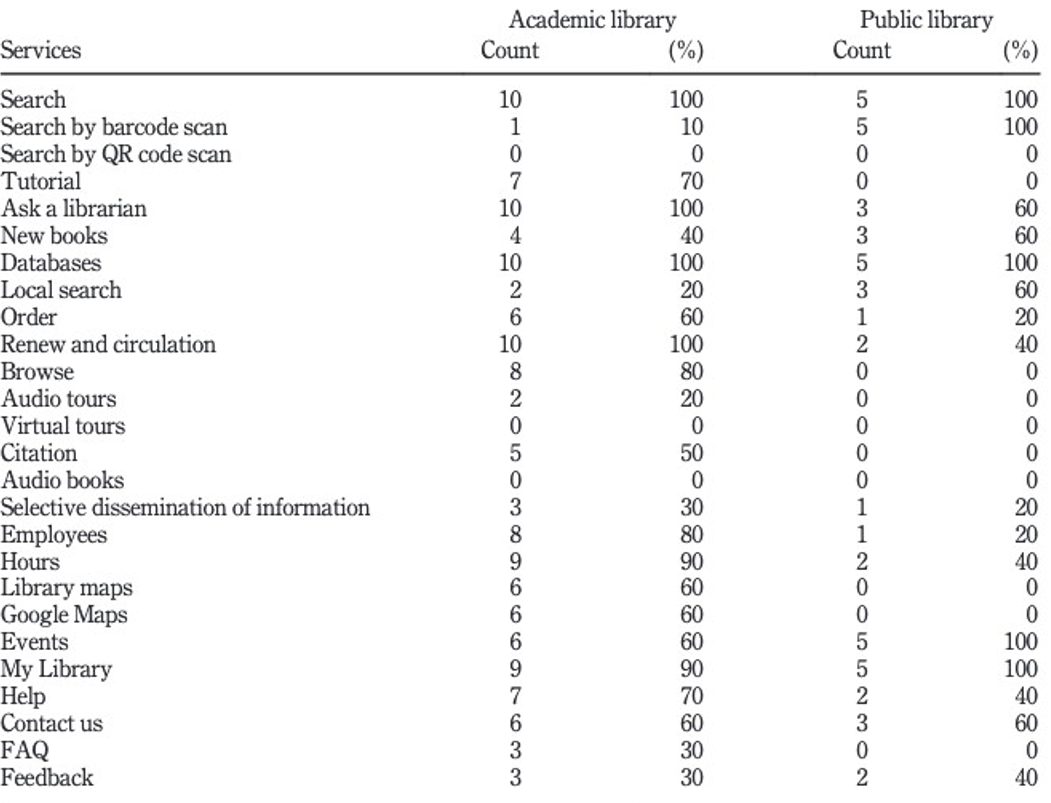
\includegraphics[width = \textwidth, height = \textheight, keepaspectratio]{assets/img/Accessing Mobile Applications.png}
        \caption{Frequency and percentage of components in library mobile applications by type of library}
        \label{fig:freq_and_per_comp_lib_mob_app}
    \end{figure}
    \noindent{} \textit{Note}: From “Assessing mobile application components in providing library services,” by A. Mansouri and N. Soleymani Asl, 2019, \textit{The Electronic Library}, 37(1), p. 53 (https://doi.org/10.1108/EL-10-2018-0204). Copyright 2019 by Emerald Publishing Limited. Reprinted with permission.
    
    
    \paragraph{}
    Figure 2.1 shows the breakdown of all services found within the library mobile applications reviewed by the study, and how frequently they were utilized. The "Public library" column is irrelevant in this report. This is a great example of a model for features that are used in the field already. Such features (see Appendix 6.3.2 for a detailed outline of each) include a search, either by barcode or QR code or both. This enriched set of features was made a common resource within each of the library applications reviewed in this study. Tutorials to help viewers to learn the platform and its capabilities for those who are perhaps new to it are yet another useful feature. The ask a librarian resource would bridge the gap between a librarian and an individual who may have questions for a librarian. A simple, yet helpful feature quite commonly seen in other library applications is the library hours. Having access to the hours of a library provides the users with much of the information they should need to utilize it. The remaining details that may be missing from the user's knowledge would be event and calendar information. Nearly every library mobile app reviewed in this study by Mansouri and Soleymani, provides such a feature. Lastly, a FAQ (Frequently Asked Questions)/Feedback element, not quite as commonly included within a library mobile application, was considered useful nonetheless.
     

%Section 2.5
\section{State of the Art}
    \paragraph{}
    Throughout the years, app development has improved in both efficiency, quality, and accessibility. As a result, library apps - as well as similar learning-based apps - have improved in these criteria congruently. One feature of modern day mobile applications is an emphasis on integration with other relevant software. For example, an Ex Libris press release about the Libris CampusM Mobile App, stated: "The flexibility of the app enables it to be integrated with learning management systems such as Blackboard®, Canvas, and Moodle™"(Ex Libris, 2017). This cross-platform paradigm is essential in applications which were built to service existing technologies and state of the art library mobile applications, and integrate with existing programs and databases. Pu et al. (2015) describes the origins of a library mobile app; "A number of libraries gradually sensed this trend and combined their services with mobile technology to created so-called Mobile Library or M-Library".(2015, p.15-31).
    \paragraph{} 
    In addition to being highly integrated with existing technology, state of the art mobile applications utilize technologies built into smartphones in order to give users the best possible experience. Hu & Neamtiu (2016) state, "The behavior of smartphone apps is driven by input from sensors such as GPS, microphone, or camera" (p.50-56). State of the art library applications also utilize the technology provided by mobile phones in order to maximize their utility. For example, a library app might use the camera in order to scan bar codes. Furthermore, a library application could utilize the GPS technology to inform users about their distance from the library. Essentially, state of the art apps, including library apps, utilize the state of the art technology features on smartphones.
    \paragraph{}
    Another feature of modern technology, particularly software, is change. State of the art applications are dynamic entities; they improve with time and require consistent maintenance (Hu \& Neamtiu, 2016). Anand et al. (2020) writes, "Thus, to keep the software and its data safe, software developers perform continuous testing of the product in its operational phase and release software upgrades or software updates/patches to fix any uprising issue and to improve it (p.1071-1085).  Essentially, state of the art software, mobile applications specifically, including library applications, are upgraded, maintained and modified on a regular basis.
    \paragraph{}
    Yet another feature of state of the art software is the ability to provide value in multiple ways. State of the art tools not only provide useful services to the clients, but also provide the client with value. With respect to library application specifically, this means the software is designed such that data can be collected from the users to exponentially improve the software. Chen (2019) notes, "This indicated that Mobile Library has become a vital resource for learners to acquire knowledge" (p.721-734).
    
    %%List here is just for information purposes. Text above is the actual thing
    
    % \begin{itemize}
    
    %     \item
    %     "The flexibility of the app enables it to be integrated with learning management systems such as Blackboard®, Canvas, and Moodle™" \cite{campusM}
    %     \item
    %     "Since the app runs on library-developed open-source software, feedback from academic users during the pilot program – currently running until August 31 – will also help develop and improve new functionality in the app, which will benefit all library users." \cite{NYU_Library}.
    %     \item
    %     "Since the app runs on library-developed open-source software, feedback from academic users during the pilot program – currently running until August 31 – will also help develop and improve new functionality in the app, which will benefit all library users." \cite{NYU_Library}.
    %     \item 
    %     "The behavior of smartphone apps is driven by input from
    %     sensors such as GPS, microphone, or camera", 
    %     "First, we fuzz (alter) the log in a semantically-meaningful way: by applying 
    %     principled transformations (e.g., changing GPS coordinates
    %     or navigation speed), a new input log is constructed, which
    %     represents a new test case. Second, we use the log captured
    %     in app A to test an app B which offers similar functionality,
    %     e.g., GPS navigation or image recognition"
    %     "For example, GPS allows apps such as Yelp to provide location-aware services; the camera allows image matching apps like Google Goggles to provide search-by-picture features; the Shazam app can help recognize an ambient song by using the microphone."
    %     \cite{FuzzyAndCross}
    %     \item
    %     With the unceasing advancement of mobile technologies, mobile devices developed rapidly. Thus, learning activities could be proceeded anytime and anywhere (Lai et al. , 2014). Wang et al. (2012) indicated that, with the popularization of 3G mobile technologies, more people gained access to internet to view web site, receive and send e-mails and read e-books with smartphones and tablet PCs on metro, bus or train. It could be inferred that learning activities no longer limit to classroom or scheduled time. By combining mobile devices and wireless technology, learning guidance and feedbacks could be given according to learners' learning situations and learning environment (Huang et al. , 2014).

    %     A number of libraries gradually sensed this trend and combined their services with mobile technology to created so-called Mobile Library or M-Library. In fact, the concept of Mobile Library or M-Library was brought up by scholars when PDAs were still in development. For instance, Janet (2009) adapted mobile technology and combined PDA with library orientation and collection search services. However, at that time, mobile devices and wireless technology were not mature and popular.
        
    %     "Recently, mobile technology combined with mobile devices has become an important information collecting channel. A greater number of students and teachers also use tablet PCs and smartphone to search for e-journals, e-books and other e-resources (Parsons, 2010). Therefore, numerous libraries introduced mobile technology in library services and developed mobile information systems compatible to mobile devices in order to allow their users quickly search for desired information (Wang et al. , 2012). This indicated that Mobile Library has become a vital resource for learners to acquire knowledge."
    %     "Ten participants reported that it was easier to search the library catalog using the laptop.They explained that they were familiar with the interface of web OPACs, and more information was displayed on the computer screen than the tablet screen"
    %     "Some participants reported that they would use the smartphone app to search library catalogs when it was inconvenient to use laptops or desktop computers, such as on the bus or in classroom"
    %     \cite{given_one}
       
    % \end{itemize}
    
    
% Section:
% 2.6
\section{Relation to the Larger Problem Area}
    \paragraph{}
     As the world becomes more digitized, and tools once only accessible in person are made accessible via the internet, projects such as this become increasingly relevant. One particular field in which modernization is occuring is mobile development. Specifically, mobile development with respect to the virtualization of already existing tools. This includes mobile apps to make delivery placements for food, mobile applications to handle transportation, and generally any service that can be digitized. According to Genuitec, an enterprise-consulting company, "The open-source community is helping to rapidly advance mobile Web application development. To date, no less than eighteen different mobile frameworks exist just for the iPhone" ("MobiOne Developer 1.0 M4", 2009). Mobile application is one of the broadest and most widely used examples of the digitization of the modern world. 
     
     \paragraph{}
     A number of factors explain this trend towards digitization via mobile applications. Firstly is the decreased cost. A major advantage of software is its repeatability. If software is developed once, it could be re-implemented as many times as desired with virtually no additional cost. Furthermore, mobile applications save users a significant amount of time; virtually any good or service is a few clicks away. Another factor in the popularization of mobile applications is the popularity of smart phones. Genuitec noted, "This time next year we expect the mobile Web to have matured significantly as smartphones get cheaper and more diverse, and desktop developers spend more energy creating applications for the computer in your pocket," ("MobiOne Developer 1.0 M4", 2009). As smartphones become more popular, digitization implemented with this software will become more popular, leading to the further popularization of smart phones. The result, then, would be a positive feedback loop between smartphones and mobile apps. 
     
     \paragraph{}
     Application development with respect to library services in particular, is a fast-growing niche. Hu & Neamtiu (2016) wrote, "Recently, mobile technology combined with mobile devices has become an important information collecting channel. A greater number of students and teachers also use tablet PCs and smartphone to search for e-journals, e-books and other e-resources" (p.50-56).
     In essence, library features become a particularly fruitful avenue for the area of the modernization and digitization of existing tools. This trend can be attributed to the data-driven services libraries provide. Libraries provide excessive amounts of data, giving developers solid materials to work with. Furthermore, libraries tend to be affiliated with higher education - often a university for example - which further increases the inclination of software developers, often affiliated with these places of higher learning, to develop mobile applications for these institutions.
     \paragraph{}
     Furthermore, mobile library-specific application development has been proven to be highly for library administrators. This is because mobile apps serve not just the function of aiding its users in whatever tasks they have been designed to aid with, but also because they can be regarded as a data collection tool for individuals overseeing the institution with which the application is connected. Therefore,  numerous  libraries  introduced  mobile technology in library services and developed mobile information systems compatible to mobile devices in order to allow their users quickly search for desired information(p.721-734). Mobile apps allow library administrators to get nearly instant feedback with regards to the various services and features offered by the library, making it a useful tool for growing and developing libraries and library services. 
    
    
    % \begin{itemize}
    %     \item 
    %     "The open-source community is helping to rapidly advance mobile Web application development. To date, no less than eighteen different mobile frameworks exist just for the iPhone. Yet few mobile Web developers know of them and their rich user interface capabilities and smart device features. MobiOne is introducing Community Insights, an integrated feature that brings together real time news and information about mobile Web frameworks with numerous examples that can be instantly loaded into the MobiOne iPhone and Palm Pre emulators for evaluation. "This time next year we expect the mobile Web to have matured significantly as smartphones get cheaper and more diverse, and desktop developers spend more energy creating applications for the computer in your pocket," said Maher Masri, president and CEO of Genuitec. "Mobile devices are becoming more prevalent and as the market grows, software developers will be armed for success with powerful tools like MobiOne.""\cite{MobiOne}
        
    %     \item
    %     There exists a trend towards mobile computing. "Gradually, many libraries sense this trend and start to ponder on methods of providing innovative services by using mobile technology". Mobile innovative services of library means that a library utilizes mobile technology to allow is readers view,search and obtain library services without being limited by time and place (Chang,2013) \cite{pu_chiu_chen_huang_2015}. In summary, libraries are attempting to offer mobile applications for their services. We want to do exactly that. We want an application that students can use wherever and whenever to access library services.
        
    %     \item
    %     "Recently, mobile technology combined with mobile devices has become an important information collecting channel. A greater number of students and teachers also use tablet PCs and smartphone to search for e-journals, e-books and other e-resources  (Parsons,  2010).  Therefore,  numerous  libraries  introduced  mobile technology in library services and developed mobile information systems compatible to mobile devices in order to allow their users quickly search for desired information(Wanget al., 2012). This indicated that Mobile Library has become a vital resource for learners to acquire knowledge" \cite{pu_chiu_chen_huang_2015}.
    %     \item
    %     Found in a study by a team from San Agustin University's Computer Science department in Peru, and among 163 surveyed students, those students mostly utilize academic apps that assist in making their academic workload easier and more efficient to handle. These such apps include: GeoGebra, Mathway, Kahn Academy, Duolingo, Symbolab, and numerous others. As we delve into the concept of creating a more ease of access system for academic resources here at WPI, this study shows just what students are wanting from mobile apps, convenience.\cite {Educational_Apps}
    % \end{itemize}
    
    
    % Section 2.7 -- INITIAL REVISIONS MADE FOR BRANDON'S SECTIONS
    \section{Closing Thoughts}
    \paragraph{}
    Mobile devices are being increasingly utilized within academic contexts. Easy access to academic library resources and services is just one need students have throughout their academic careers. As this need is still in its infancy, little is known about mobile library applications specifically. However, much is known about the development of standard mobile applications and the requirements of a mobile app. Based on research in this field, connections and patterns were drawn between the state of the art library applications. An example pattern was how mobile applications are often integrated with the already existing library features; as opposed to developing features from scratch, they built on the existing tools offered by libraries.